\section[\appendixname~\thesection]{Bandwise Grayscale Reconstructions}
\label{appendix:bandwise_results}

\begin{figure}[H]
\begin{adjustwidth}{-\extralength}{0cm}
\centering

\subfloat[\centering Band 1]{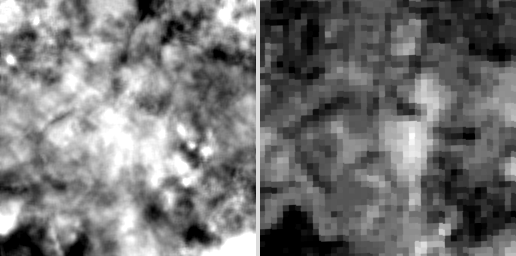
\includegraphics[width=6.0cm]{img/bands_gray/sample_000008_B01_panel.png}}
\hfill
\subfloat[\centering Band 2]{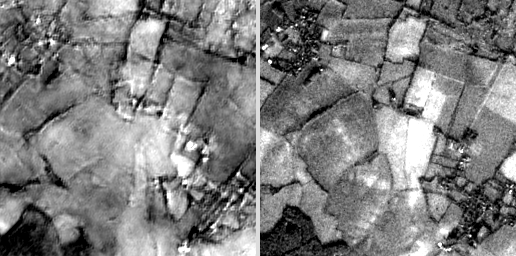
\includegraphics[width=6.0cm]{img/bands_gray/sample_000008_B02_panel.png}}
\hfill
\subfloat[\centering Band 3]{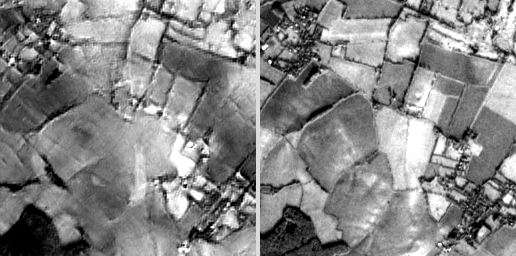
\includegraphics[width=6.0cm]{img/bands_gray/sample_000008_B03_panel.png}}\\

\subfloat[\centering Band 4]{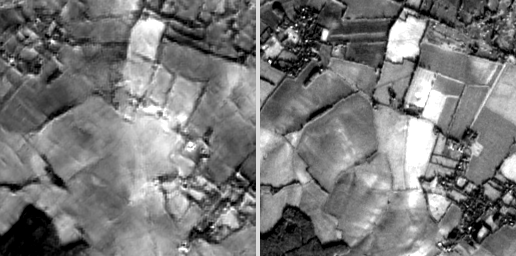
\includegraphics[width=6.0cm]{img/bands_gray/sample_000008_B04_panel.png}}
\hfill
\subfloat[\centering Band 5]{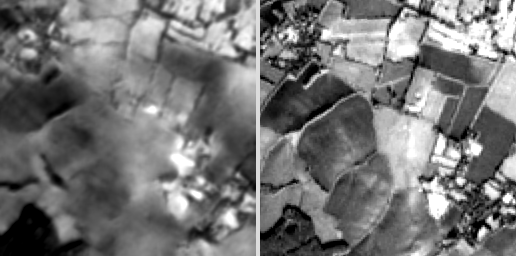
\includegraphics[width=6.0cm]{img/bands_gray/sample_000008_B05_panel.png}}
\hfill
\subfloat[\centering Band 6]{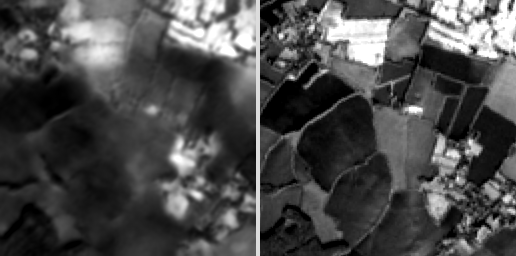
\includegraphics[width=6.0cm]{img/bands_gray/sample_000008_B06_panel.png}}\\

\subfloat[\centering Band 7]{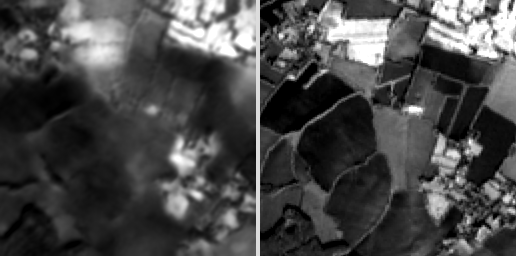
\includegraphics[width=6.0cm]{img/bands_gray/sample_000008_B07_panel.png}}
\hfill
\subfloat[\centering Band 8]{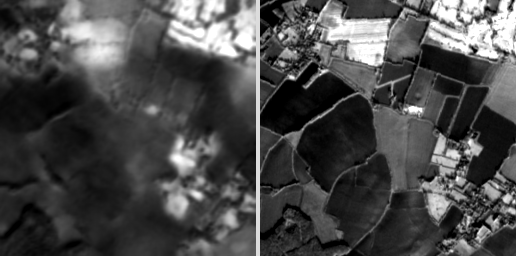
\includegraphics[width=6.0cm]{img/bands_gray/sample_000008_B08_panel.png}}
\hfill
\subfloat[\centering Band 8A]{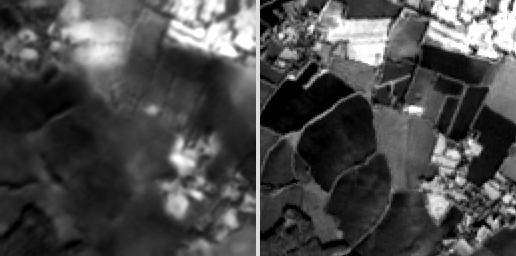
\includegraphics[width=6.0cm]{img/bands_gray/sample_000008_B09_panel.png}}\\

\subfloat[\centering Band 9]{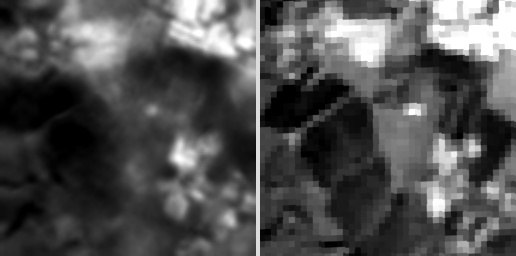
\includegraphics[width=6.0cm]{img/bands_gray/sample_000008_B10_panel.png}}
\hfill
\subfloat[\centering Band 10]{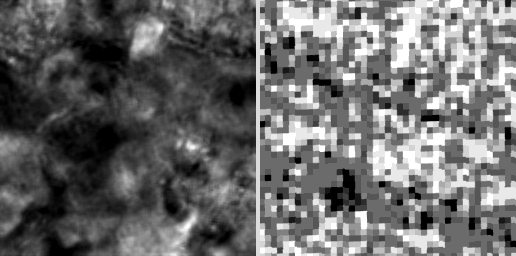
\includegraphics[width=6.0cm]{img/bands_gray/sample_000008_B11_panel.png}}
\hfill
\subfloat[\centering Band 11]{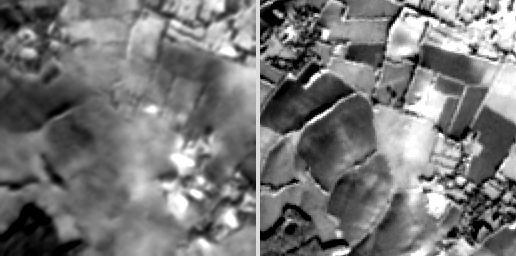
\includegraphics[width=6.0cm]{img/bands_gray/sample_000008_B12_panel.png}}\\

\subfloat[\centering Band 12]{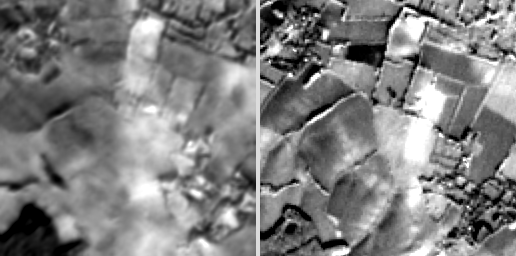
\includegraphics[width=6.0cm]{img/bands_gray/sample_000008_B13_panel.png}}

\end{adjustwidth}
\caption{Bandwise grayscale reconstructions for all Sentinel-2 bands. For all bands: generated left, ground truth right.\label{appendix_fig}}
\end{figure} 

